% !TeX root = enterprise-architecture-digital-blueprint.tex
% !TeX encoding = UTF-8
\chapter{Kerangka Kerja Arsitektur: TOGAF, Zachman, dan Arsitektur SPBE}

\section*{Tujuan Pembelajaran}
\begin{itemize}
  \item Menjelaskan struktur TOGAF Standard edisi ke-10 dan urutan fase ADM (\textit{Architecture Development Method}).
  \item Membandingkan TOGAF, Zachman Framework, dan Arsitektur SPBE (Sistem Pemerintahan Berbasis Elektronik) dari sisi tujuan, cakupan, dan cara pakai.
  \item Menyusun peta pemangku kepentingan beserta \textit{concern} dan ruang lingkup kerja arsitektur.
\end{itemize}

\section{Pendahuluan}

Organisasi yang sudah beberapa kali menyewa konsultan biasanya menyimpan
beberapa dokumen arsitektur sekaligus. Dokumen dari vendor SIMRS (Sistem
Informasi Manajemen Rumah Sakit) berisi diagram server dan basis data.
Dokumen dari konsultan yang memasang ERP (\textit{Enterprise Resource
Planning}) keuangan berisi peta proses dan daftar laporan. Dokumen dari tim
internal berisi daftar aplikasi dengan kolom yang berbeda lagi. Ketiganya
menggambarkan organisasi yang sama, tetapi tidak dapat diletakkan
berdampingan. Istilahnya berbeda, tingkat rinciannya berbeda, dan tidak ada
yang tahu bagian mana yang belum digambar sama sekali.

Kondisi ini punya tiga akibat. Pertama, dokumen sulit dibandingkan, sehingga
direksi tidak dapat menilai usulan mana yang lebih baik. Kedua,
kelengkapannya sulit diperiksa, karena tidak ada daftar tentang apa saja
yang seharusnya ada. Ketiga, hasil kerja sulit dipakai ulang, sehingga setiap
proyek baru mulai menggambar dari nol. Kerangka kerja arsitektur menjawab
ketiga masalah itu dengan menyediakan kosakata, susunan isi, dan urutan kerja
yang disepakati bersama. Bab 1 sudah memperkenalkan arsitektur
\textit{enterprise} (\textit{Enterprise Architecture}, EA) sebagai praktik.
Bab ini membahas alat bantunya.

Pembahasan dimulai dari kosakata dasar menurut standar ISO/IEC/IEEE
42010:2022, terbitan bersama International Organization for Standardization
(ISO), International Electrotechnical Commission (IEC), dan Institute of
Electrical and Electronics Engineers (IEEE) \cite{iso42010}. Sesudahnya
dibahas TOGAF (\textit{The Open Group Architecture Framework}) Standard edisi
ke-10 sebagai metode dan susunan isi \cite{togaf10, c02-togaf-pocket},
Zachman Framework sebagai skema klasifikasi \cite{zachman1987, c02-sowa1992},
dan Arsitektur SPBE sebagai kerangka yang diwajibkan bagi instansi pemerintah
\cite{perpres95-2018, perpres132-2022}. Bab ditutup dengan cara menyesuaikan
kerangka untuk organisasi nyata, merujuk temuan Kotusev tentang artefak yang
benar-benar dipakai \cite{kotusev2019}, lalu dengan Aktivitas yang
menghasilkan peta pemangku kepentingan dan \textit{Statement of Architecture
Work} untuk tonggak C1.

\IfFileExists{../figures/ch02-diagram-konsep.png}{%

Gambar \ref{fig:ch02-ilustrasi-bab} merangkum hubungan komponen dan konsep utama bab ini.
\begin{figure}[!htb]
  \centering
  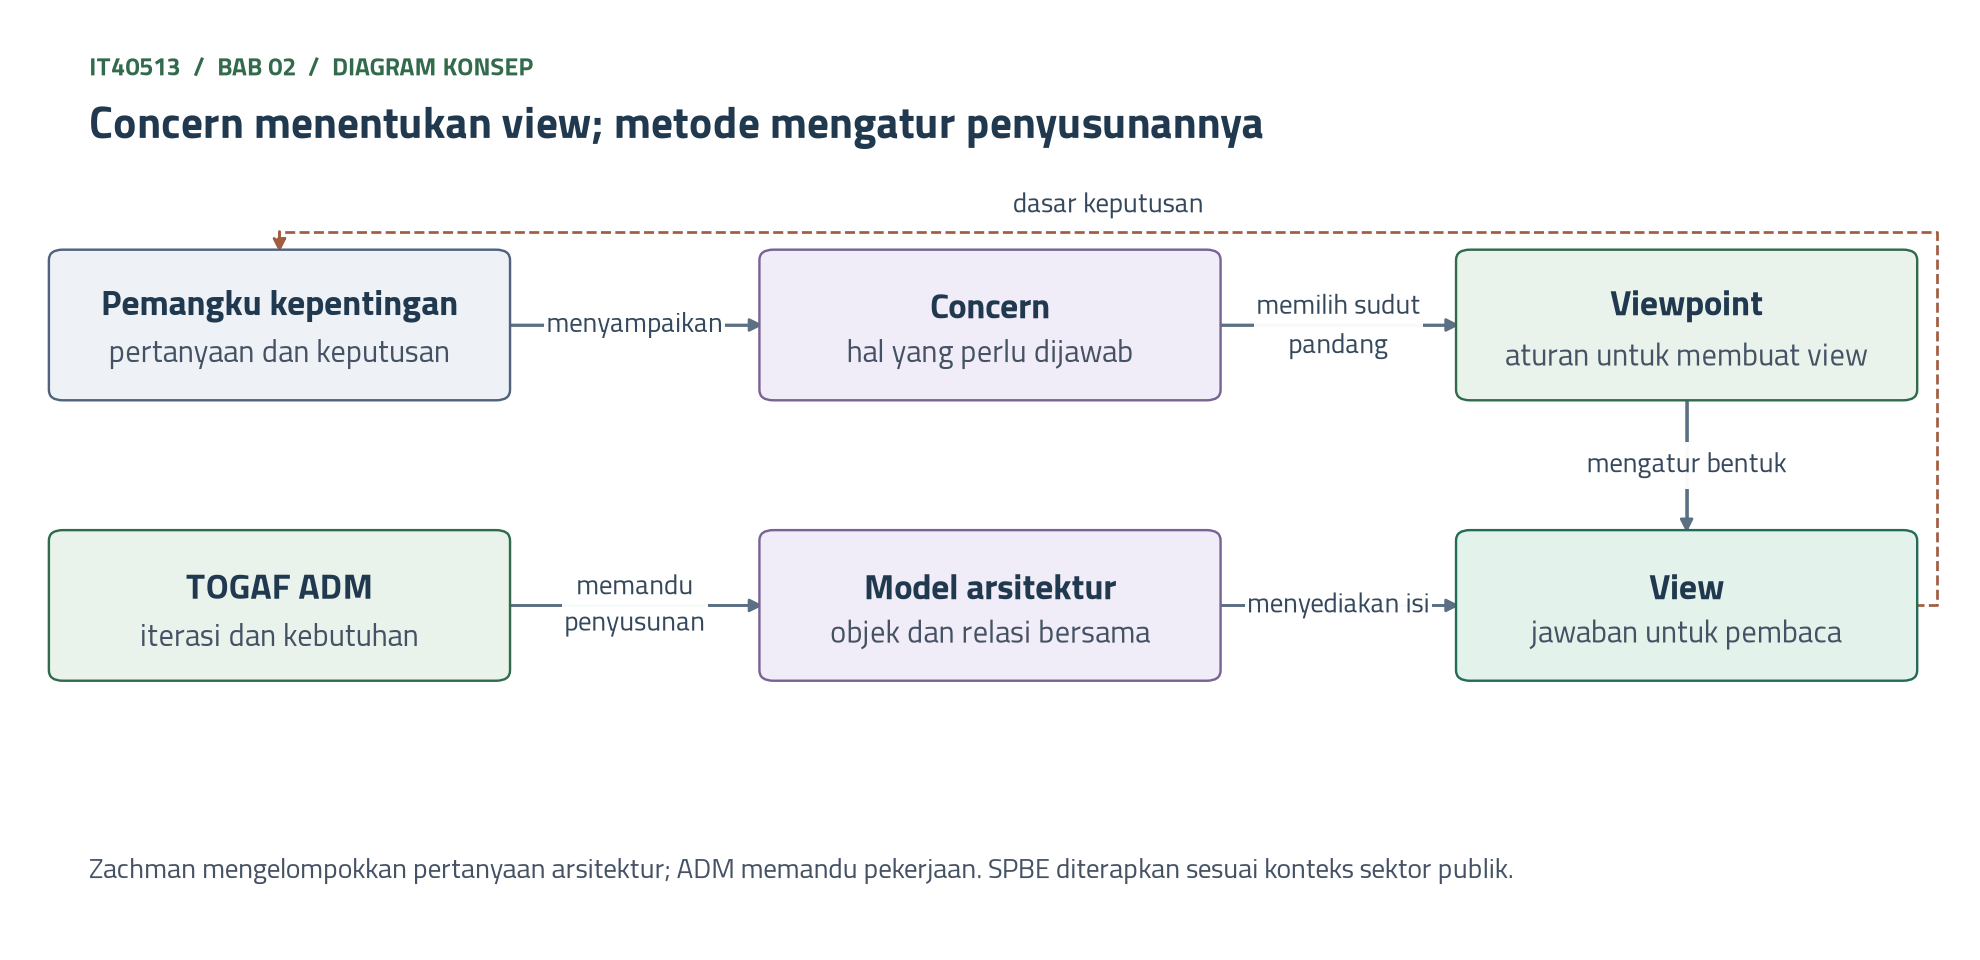
\includegraphics[width=\textwidth]{../figures/ch02-diagram-konsep.png}
  \caption{Concern menentukan view; metode mengatur penyusunannya}
  \label{fig:ch02-ilustrasi-bab}
\end{figure}
}{}

\section{Stakeholder, Concern, View, dan Viewpoint}

Ketiga dokumen pada Pendahuluan berbeda bukan karena penulisnya ceroboh.
Masing-masing ditulis untuk pembaca yang berbeda dan menjawab pertanyaan yang
berbeda, tetapi tidak satu pun menuliskan untuk siapa dan untuk pertanyaan
apa dokumen itu dibuat. Standar ISO/IEC/IEEE 42010:2022 menutup celah
tersebut. Standar ini tidak mengatur cara merancang arsitektur, melainkan isi
minimum sebuah deskripsi arsitektur, sehingga deskripsi buatan tim mana pun
dapat dibaca dan diperiksa dengan cara yang sama \cite{iso42010}.

Standar ini membedakan arsitektur dari deskripsi arsitektur. Arsitektur
adalah konsep dan sifat mendasar sebuah entitas di dalam lingkungannya,
beserta prinsip yang mengarahkan perwujudan dan perubahannya. Deskripsi
arsitektur adalah produk kerja yang mengungkapkan arsitektur itu, misalnya
dokumen, model, atau isi repositori. Arsitektur tetap ada walaupun tidak
pernah ditulis, tetapi yang dapat diperiksa dan dibandingkan hanya
deskripsinya. Edisi 2022 menyebut objek yang dikaji sebagai \textit{entity of
interest}, menggantikan \textit{system of interest} pada edisi 2011, karena
objek itu tidak harus berupa sistem perangkat lunak. Objek itu dapat berupa
satu organisasi, satu jaringan rumah sakit, atau satu layanan.

Empat konsep inti menyusul dari pembedaan tersebut:

\begin{itemize}
  \item \textbf{Pemangku kepentingan} (\textit{stakeholder}) adalah orang,
        kelompok, atau organisasi yang berkepentingan atas entitas yang
        dikaji.
  \item \textbf{\textit{Concern}} adalah kepentingan atau pertanyaan pemangku
        kepentingan terhadap entitas itu, misalnya biaya, keamanan data,
        waktu tunggu, atau kepatuhan pada regulasi.
  \item \textbf{\textit{View}} adalah bagian deskripsi arsitektur yang
        menjawab satu atau beberapa \textit{concern} tertentu.
  \item \textbf{\textit{Viewpoint}} adalah aturan untuk membuat dan membaca
        sebuah \textit{view}: \textit{concern} apa yang dijawab, untuk
        pemangku kepentingan mana, jenis model apa yang dipakai, dan
        notasinya.
\end{itemize}

Gambar \ref{fig:ch02-konsep-42010} merangkai keempatnya. Pemangku
kepentingan memiliki \textit{concern}, \textit{viewpoint} membingkai
\textit{concern} itu dan mengatur cara membuat \textit{view}, lalu
\textit{view} yang termuat di deskripsi arsitektur menjawab \textit{concern}
tersebut.

\begin{figure}[!htb]
  \centering
  \begin{tikzpicture}[
  font=\scriptsize,
  kotak/.style={draw, rounded corners, minimum height=0.95cm, minimum width=2.7cm,
                align=center, font=\scriptsize\bfseries},
  panah/.style={-{Stealth[length=2mm]}, thick},
  ket/.style={font=\tiny, fill=white, inner sep=1pt}
]
  \node[kotak, fill=praditagreen!15] (entitas) at (0,0)
    {Entitas yang dikaji\\{\tiny\mdseries\textit{entity of interest}}};
  \node[kotak, fill=blue!8] (arsitektur) at (4.4,0)
    {Arsitektur\\{\tiny\mdseries ada walau tak ditulis}};
  \node[kotak, fill=green!10] (deskripsi) at (8.8,0)
    {Deskripsi arsitektur\\{\tiny\mdseries dokumen, model}};

  \node[kotak, fill=blue!8] (pemangku) at (0,-2.4)
    {Pemangku kepentingan\\{\tiny\mdseries\textit{stakeholder}}};
  \node[kotak, fill=orange!12] (concern) at (4.4,-2.4)
    {Concern\\{\tiny\mdseries kepentingan, pertanyaan}};
  \node[kotak, fill=green!10] (view) at (8.8,-2.4)
    {View\\{\tiny\mdseries gambar yang menjawab}};

  \node[kotak, fill=blue!8] (viewpoint) at (6.6,-4.6)
    {Viewpoint\\{\tiny\mdseries aturan membuat view}};

  \draw[panah] (entitas) -- node[ket, above] {memiliki} (arsitektur);
  \draw[panah] (arsitektur) -- node[ket, above] {diungkapkan dalam} (deskripsi);
  \draw[panah] (pemangku) -- node[ket, right] {berkepentingan pada} (entitas);
  \draw[panah] (pemangku) -- node[ket, above] {memiliki} (concern);
  \draw[panah] (deskripsi) -- node[ket, right] {memuat} (view);
  \draw[panah] (view) -- node[ket, above] {menjawab} (concern);
  \draw[panah] (viewpoint.west) -| node[ket, pos=0.75, left] {membingkai} (concern.south);
  \draw[panah] (viewpoint.east) -| node[ket, pos=0.75, right] {mengatur} (view.south);
\end{tikzpicture}

  \caption{Konsep inti ISO/IEC/IEEE 42010:2022: setiap \textit{view} ada
           karena ada \textit{concern} yang harus dijawab}
  \label{fig:ch02-konsep-42010}
\end{figure}

Analoginya seperti gambar kerja sebuah gedung rumah sakit. Gedungnya satu,
tetapi gambarnya banyak. Direksi membaca denah ruang untuk melihat letak
poliklinik dan kamar rawat. Teknisi listrik membaca gambar instalasi listrik.
Petugas keselamatan membaca denah jalur evakuasi. Setiap gambar benar, tetapi
masing-masing hanya berguna bagi pembacanya. Setiap gambar adalah sebuah
\textit{view}, sedangkan aturan menggambarnya, yaitu simbol, skala, dan
legenda yang baku, adalah \textit{viewpoint}.

Dua contoh dari Medikara Health memperlihatkan cara kerjanya:

\begin{enumerate}
  \item Direktur Keuangan bertanya berapa biaya pemeliharaan integrasi per
        tahun dan integrasi mana yang paling mahal. \textit{View} yang
        menjawabnya adalah tabel biaya per antarmuka beserta trennya selama
        tiga tahun. Diagram server setebal 40 halaman tidak menjawab
        \textit{concern} itu, walaupun seluruh isinya benar.
  \item Seorang dokter di rumah sakit Bogor bertanya apakah riwayat alergi
        pasien yang pernah dirawat di Jakarta dapat dibuka saat pemeriksaan.
        Misalkan saat ini riwayat itu baru diperoleh lewat telepon ke rumah
        sakit asal, dengan waktu tunggu 15 sampai 30 menit. \textit{View}
        yang cocok adalah alur informasi pasien lintas lima rumah sakit,
        bukan daftar aplikasi.
\end{enumerate}

Dua hal pada konsep ini sering tertukar. Pembagiannya begini.
\textit{Viewpoint} bersifat umum dan dapat dipakai ulang, seperti templat
gambar instalasi listrik yang berlaku untuk gedung mana pun. \textit{View}
bersifat khusus, seperti gambar instalasi listrik untuk satu gedung tertentu.
ArchiMate menyediakan sejumlah \textit{viewpoint} siap pakai, dan Bab 4
memakainya untuk membuat \textit{view} Medikara.

\subsection*{Matriks kekuasaan dan kepentingan}

Pertanyaan kemudian muncul: pemangku kepentingan mana yang didahulukan? Tim
arsitektur tidak punya waktu untuk melayani semua \textit{concern} dengan
kedalaman yang sama. TOGAF menyediakan teknik manajemen pemangku kepentingan
dengan empat langkah: mengenali pemangku kepentingan, mengelompokkan
posisinya, menentukan cara melibatkannya, dan menyesuaikan produk kerja
untuk tiap kelompok \cite{c02-togaf-pocket}. Alat pengelompokannya adalah
matriks kekuasaan dan kepentingan. Sumbu kekuasaan mengukur kemampuan
menyetujui, menghentikan, atau mendanai. Sumbu kepentingan mengukur seberapa
besar pekerjaan arsitektur mengubah keadaan pemangku kepentingan itu.

Gambar \ref{fig:ch02-matriks-pemangku} memperlihatkan hasilnya untuk
Medikara. Pemain kunci di kanan atas dilibatkan sejak awal dan diajak
memutuskan. Pihak berkuasa di kiri atas cukup dijaga kepuasannya. Pihak yang
terdampak tetapi tidak memutuskan di kanan bawah diberi informasi rutin, dan
sisanya cukup dipantau.

\begin{figure}[!htb]
  \centering
  \begin{tikzpicture}[
  font=\scriptsize,
  judul/.style={font=\scriptsize\bfseries, anchor=north west},
  isi/.style={font=\scriptsize, anchor=north west, align=left, text width=4.6cm},
  panah/.style={-{Stealth[length=2mm]}, thick}
]
  % Empat kuadran: sumbu x kepentingan, sumbu y kekuasaan.
  \draw[fill=blue!8] (0,3.1) rectangle (5.2,6.2);
  \draw[fill=orange!12] (5.2,3.1) rectangle (10.4,6.2);
  \draw[fill=white] (0,0) rectangle (5.2,3.1);
  \draw[fill=blue!8] (5.2,0) rectangle (10.4,3.1);

  \node[judul] at (0.15,6.05) {Jaga kepuasannya {\tiny\mdseries(\textit{keep satisfied})}};
  \node[isi] at (0.15,5.55) {Dewan Komisaris\\Kementerian Kesehatan\\BPJS Kesehatan};

  \node[judul] at (5.35,6.05) {Pemain kunci {\tiny\mdseries(\textit{key players})}};
  \node[isi] at (5.35,5.55) {Direksi dan Direktur Keuangan\\Kepala TI\\Kepala lima rumah sakit\\Komite medik};

  \node[judul] at (0.15,2.95) {Pantau seperlunya {\tiny\mdseries(\textit{minimal effort})}};
  \node[isi] at (0.15,2.45) {Calon mitra ekosistem\\Perusahaan klien layanan\\kesehatan karyawan};

  \node[judul] at (5.35,2.95) {Beri informasi rutin {\tiny\mdseries(\textit{keep informed})}};
  \node[isi] at (5.35,2.45) {Dokter dan perawat\\Petugas pendaftaran\\Pasien pengguna Medikara+\\Vendor SIMRS dan Medikara+};

  % Sumbu.
  \draw[panah] (0,-0.25) -- (10.4,-0.25);
  \node[font=\tiny, anchor=north] at (5.2,-0.3) {kepentingan atas cetak biru: rendah ke tinggi};
  \draw[panah] (-0.25,0) -- (-0.25,6.2);
  \node[font=\tiny, anchor=south, rotate=90] at (-0.3,3.1) {kekuasaan atas keputusan: rendah ke tinggi};
\end{tikzpicture}

  \caption{Matriks kekuasaan dan kepentingan untuk cetak biru Medikara.
           Penempatan ini adalah contoh awal yang harus diuji lewat
           wawancara}
  \label{fig:ch02-matriks-pemangku}
\end{figure}

Penempatan ini punya dua konsekuensi. Pertama, pemangku kepentingan yang
berbeda kuadran menerima produk yang berbeda. Direksi menerima ringkasan satu
halaman dan diundang ke rapat keputusan, sedangkan petugas pendaftaran
menerima penjelasan tentang perubahan cara kerjanya. Kedua, posisi pada
matriks tidak tetap. Ackermann dan Eden menunjukkan bahwa pengelolaan
pemangku kepentingan juga dapat bertujuan mengubah posisi, misalnya
menaikkan kepentingan pihak berkuasa yang belum peduli
\cite{c02-ackermann2011}. Dewan Komisaris Medikara berada di kiri atas hari
ini, tetapi dapat pindah ke kanan atas begitu anggaran 2027 dibahas.

\begin{kasus}[title={Kasus Medikara Health: Siapa Berkepentingan atas Cetak Biru}]
\setlength{\parskip}{0.4em}
Medikara menjalankan 36 fasilitas: 5 rumah sakit, 18 klinik pratama, 1
laboratorium rujukan, dan 12 apotek. Sekitar 4.800 karyawan melayani sekitar
1,2 juta kunjungan pasien per tahun, atau rata-rata sekitar 3.300 kunjungan
per hari. Dengan skala itu, daftar pemangku kepentingan tidak dapat disusun
dari ingatan. Tim arsitektur menyusunnya dari bagan organisasi, daftar
kontrak dengan pihak luar, dan daftar regulator yang mengirim aturan dalam
tiga tahun terakhir. Hasilnya sepuluh kelompok pada
Tabel \ref{tab:ch02-concern-medikara}, dari direksi dan kepala teknologi
informasi (TI) sampai vendor.

Tiap \textit{concern} ditulis sebagai pertanyaan yang dapat dijawab dengan
data. ``Sistem yang lebih baik'' bukan \textit{concern}. ``Berapa aplikasi
yang harus dibuka untuk mendaftarkan satu pasien?'' adalah \textit{concern},
karena jawabannya dapat dihitung sebelum dan sesudah perubahan. Dua kelompok
berasal dari luar Medikara, yaitu BPJS (Badan Penyelenggara Jaminan Sosial)
Kesehatan dan Kementerian Kesehatan. Keduanya tidak ikut menyusun cetak biru,
tetapi aturannya membatasi pilihan arsitektur. Insiden kebocoran data lewat
vendor pada 2025 juga menjadikan vendor pemangku kepentingan yang
\textit{concern}-nya perlu dicatat, bukan sekadar pemasok.
\end{kasus}

\begin{table}[!htb]
  \centering
  \caption{Pemangku kepentingan Medikara, \textit{concern} utamanya, dan
           \textit{view} yang menjawabnya}
  \label{tab:ch02-concern-medikara}
  {\footnotesize
  \begin{tabularx}{\textwidth}{>{\raggedright\arraybackslash}p{2.3cm}
                               >{\raggedright\arraybackslash}X
                               >{\raggedright\arraybackslash}p{3.7cm}}
    \hline
    \textbf{Pemangku kepentingan} & \textbf{\textit{Concern} utama} & \textbf{\textit{View} yang menjawab} \\
    \hline
    Direksi & Apakah ``Satu Pasien, Satu Rekam Medis'' tercapai pada 2030, dan berapa biayanya? & Peta jalan satu halaman dengan biaya per tahun \\
    \hline
    Direktur Keuangan & Berapa biaya integrasi per tahun, dan integrasi mana yang paling mahal? & Tabel biaya per antarmuka dan trennya \\
    \hline
    Kepala rumah sakit & Apakah antrean berkurang tanpa menghilangkan keleluasaan lokal? & \textit{Value stream} rawat jalan dengan waktu tunggu \\
    \hline
    Dokter dan komite medik & Apakah riwayat pasien dari rumah sakit lain dapat dibuka saat pemeriksaan? & Alur informasi pasien lintas rumah sakit \\
    \hline
    Petugas pendaftaran & Berapa aplikasi yang harus dibuka untuk satu pasien? & Peta aplikasi per tahap pendaftaran \\
    \hline
    Pasien & Apakah data pribadi aman, dan apakah identitas tidak perlu diisi ulang? & Alur data pribadi dan titik persetujuan \\
    \hline
    BPJS Kesehatan & Apakah klaim dikirim lengkap, tepat waktu, dan sesuai ketentuan? & Alur klaim dari layanan sampai pengajuan \\
    \hline
    Kementerian Kesehatan & Apakah data layanan terkirim ke SATUSEHAT sesuai standar yang ditetapkan? & Peta antarmuka ke SATUSEHAT \\
    \hline
    Kepala TI & Berapa integrasi \textit{point-to-point} yang ada, dan siapa yang punya akses ke data pasien? & Diagram integrasi dan matriks peran akses \\
    \hline
    Vendor & Bagian kontrak mana yang berubah, dan kapan? & Status tiap aplikasi di peta jalan \\
    \hline
  \end{tabularx}}
\end{table}

\section{Struktur TOGAF Standard Edisi Ke-10}

Kosakata saja belum cukup. Tim arsitektur juga membutuhkan urutan kerja dan
daftar produk yang lazim dihasilkan, dan TOGAF Standard menyediakan keduanya.
Standar ini diterbitkan oleh The Open Group, sebuah konsorsium industri, dan
edisi ke-10 terbit pada 2022. Edisi ini dibagi menjadi dua bagian besar
\cite{togaf10}. \textit{Fundamental Content} memuat konsep dan praktik inti
yang dianggap berlaku umum, sehingga jarang berubah. \textit{Series Guides}
memberi panduan untuk menyesuaikan isi inti itu dengan topik atau konteks
tertentu, misalnya arsitektur bisnis, keamanan, atau organisasi yang bekerja
secara lincah, sehingga diperbarui lebih sering \cite{c02-togaf-pocket}.
Pembaruan Juni 2025 tidak mengubah susunan itu. Pembaruan tersebut memasukkan
\textit{Technical Corrigendum} 1 bertanggal Mei 2025, yaitu kumpulan
perbaikan dan penjelasan atas teks edisi ke-10 \cite{c02-togaf-pocket}.
Tabel \ref{tab:ch02-togaf-struktur} merangkum isi kedua bagian.

\begin{table}[!htb]
  \centering
  \caption{Susunan TOGAF Standard edisi ke-10, pembaruan 2025}
  \label{tab:ch02-togaf-struktur}
  {\footnotesize
  \begin{tabularx}{\textwidth}{>{\raggedright\arraybackslash}p{2.0cm}
                               >{\raggedright\arraybackslash}p{4.0cm}
                               >{\raggedright\arraybackslash}X}
    \hline
    \textbf{Bagian} & \textbf{Dokumen} & \textbf{Isi pokok} \\
    \hline
    \textit{Fundamental Content} & \textit{Introduction and Core Concepts} & Pengertian EA, konsep inti, istilah, dan cara membaca standar \\
    \hline
     & \textit{Architecture Development Method} & Fase ADM beserta tujuan, langkah, masukan, dan luarannya \\
    \hline
     & \textit{ADM Techniques} & Manajemen pemangku kepentingan, \textit{gap analysis}, manajemen risiko, serta alternatif dan \textit{tradeoff} \\
    \hline
     & \textit{Applying the ADM} & Iterasi, gaya arsitektur, dan pembagian lanskap arsitektur \\
    \hline
     & \textit{Architecture Content} & Kerangka isi, produk kerja, \textit{Enterprise Continuum}, dan \textit{Architecture Repository} \\
    \hline
     & \textit{Enterprise Architecture Capability and Governance} & Membangun kapabilitas arsitektur, tata kelola, dan \textit{architecture board} \\
    \hline
    \textit{Series Guides} & Contoh: arsitektur bisnis, keamanan, data dan informasi, metode lincah, model referensi pemerintahan & Panduan menyesuaikan isi inti untuk topik atau konteks tertentu \\
    \hline
  \end{tabularx}}
\end{table}

Analoginya seperti dapur jaringan rumah makan waralaba. Dapur pusat punya
buku standar yang jarang berubah: cara menyimpan bahan, urutan memasak, dan
ukuran porsi. Di samping itu ada panduan menu musiman dan menu daerah yang
diganti beberapa kali setahun. Cabang mana pun memakai buku standar yang
sama, lalu memilih panduan yang sesuai dengan pelanggannya.

Dua contoh pemakaiannya:

\begin{enumerate}
  \item Tim \textit{capstone} dengan 14 pertemuan tidak membaca keenam
        dokumen \textit{Fundamental Content} sekaligus. Bab ini memakai
        dua, yaitu \textit{Architecture Development Method} dan bagian
        manajemen pemangku kepentingan dari \textit{ADM Techniques}. Bab 14
        memakai dokumen keenam tentang tata kelola.
  \item Tim internal Medikara yang menyusun \textit{capability map} untuk
        lima rumah sakit memakai \textit{Series Guide} arsitektur bisnis,
        karena panduan langkah demi langkahnya ada di sana. Bab 5
        membahasnya bersama BIZBOK.
\end{enumerate}

\subsection*{Deliverable, artefak, dan building block}

Tiga istilah dalam TOGAF sering tertukar. Pembagiannya begini.
\textit{Deliverable} adalah produk kerja yang disepakati dalam rencana
kerja, ditinjau secara formal, lalu disetujui pemangku kepentingan.
Artefak adalah produk kerja yang menggambarkan satu sisi arsitektur, dengan
tiga bentuk: katalog berupa daftar, matriks berupa hubungan antara dua
daftar, dan diagram berupa gambar. Satu \textit{deliverable} biasanya berisi
beberapa artefak. \textit{Building block} adalah komponen kapabilitas
organisasi yang dapat dipakai ulang dan digabungkan dengan komponen lain.
\textit{Architecture building block} menyatakan apa yang dibutuhkan,
sedangkan \textit{solution building block} menyatakan produk atau komponen
nyata yang memenuhinya \cite{togaf10}.

Analoginya seperti membangun rumah. Berkas persetujuan bangunan yang
ditandatangani pejabat berwenang adalah \textit{deliverable}. Denah, daftar
bahan, dan tabel kebutuhan listrik per ruangan adalah artefak berbentuk
diagram, katalog, dan matriks. Spesifikasi ``kusen pintu 80 kali 210
sentimeter'' adalah \textit{architecture building block}, sedangkan kusen
merek tertentu yang dibeli di toko adalah \textit{solution building block}.
Tabel \ref{tab:ch02-tiga-istilah} memindahkan pembagian itu ke Medikara.

\begin{table}[!htb]
  \centering
  \caption{Tiga istilah TOGAF yang sering tertukar, dengan contoh Medikara}
  \label{tab:ch02-tiga-istilah}
  {\footnotesize
  \begin{tabularx}{\textwidth}{>{\raggedright\arraybackslash}p{2.6cm}
                               >{\raggedright\arraybackslash}p{3.8cm}
                               >{\raggedright\arraybackslash}X}
    \hline
    \textbf{Istilah} & \textbf{Ciri} & \textbf{Contoh Medikara} \\
    \hline
    \textit{Deliverable} & Disepakati, ditinjau formal, disetujui & \textit{Statement of Architecture Work} yang ditandatangani direksi \\
    \hline
    Artefak: katalog & Daftar unsur sejenis & Katalog aplikasi di 36 fasilitas \\
    \hline
    Artefak: matriks & Hubungan antara dua daftar & Matriks aplikasi lawan kapabilitas bisnis \\
    \hline
    Artefak: diagram & Gambar susunan dan hubungan & Diagram integrasi SIMRS, ERP, Medikara+, BPJS Kesehatan, dan SATUSEHAT \\
    \hline
    \textit{Architecture building block} & Kebutuhan yang dapat dipakai ulang, belum terikat produk & Layanan identitas pasien tunggal untuk seluruh fasilitas \\
    \hline
    \textit{Solution building block} & Produk atau komponen nyata & Produk pengelola identitas pasien yang dipilih pada Bab 9 \\
    \hline
  \end{tabularx}}
\end{table}

Dua istilah lain melengkapi susunan isi TOGAF. \textit{Enterprise
Continuum} mengelompokkan arsitektur dan solusi dari yang paling umum sampai
yang paling khusus: arsitektur fondasi, arsitektur sistem umum, arsitektur
industri, dan arsitektur khusus organisasi. Standar HL7 (\textit{Health
Level Seven}) FHIR (\textit{Fast Healthcare Interoperability Resources}) yang
dipakai SATUSEHAT berada di tingkat industri kesehatan, sedangkan rancangan
integrasi Medikara berada di tingkat khusus organisasi. \textit{Architecture
Repository} adalah tempat menyimpan seluruh hasil kerja itu: lanskap
arsitektur saat ini dan target, standar, model referensi, dan catatan
keputusan tata kelola \cite{togaf10}. Bab 14 membahas cara memeliharanya.

\section{Siklus ADM}

ADM adalah metode inti TOGAF. Metode ini terdiri atas fase
\textit{Preliminary}, delapan fase berlabel A sampai H, dan Manajemen
Kebutuhan (\textit{Requirements Management}) di tengah siklus. Setiap fase
punya tujuan, masukan, langkah, dan luaran. Luaran satu fase menjadi masukan
fase berikutnya, sedangkan Manajemen Kebutuhan menampung kebutuhan baru yang
muncul kapan saja dan menilai dampaknya ke fase yang sedang berjalan
\cite{togaf10, c02-togaf-pocket}. Gambar \ref{fig:ch02-siklus-adm}
memperlihatkan siklusnya.

\begin{figure}[!htb]
  \centering
  \begin{tikzpicture}[
  font=\scriptsize,
  fase/.style={draw, rounded corners, minimum height=0.95cm, minimum width=2.45cm,
               align=center, font=\scriptsize},
  panah/.style={-{Stealth[length=2mm]}, thick},
  dua/.style={{Stealth[length=1.5mm]}-{Stealth[length=1.5mm]}, gray}
]
  \node[fase, fill=orange!12] (pre) at (0,4.05)
    {\textbf{Preliminary}\\{\tiny persiapan dan prinsip}};
  \node[fase, fill=orange!12] (a) at (0,2.55) {\textbf{A}\\{\tiny visi arsitektur}};
  \node[fase, fill=blue!8] (b) at (3.15,1.65) {\textbf{B}\\{\tiny arsitektur bisnis}};
  \node[fase, fill=blue!8] (c) at (4.0,0) {\textbf{C}\\{\tiny arsitektur sistem}\\{\tiny informasi}};
  \node[fase, fill=blue!8] (d) at (3.15,-1.65) {\textbf{D}\\{\tiny arsitektur teknologi}};
  \node[fase, fill=green!10] (e) at (0,-2.55) {\textbf{E}\\{\tiny peluang dan solusi}};
  \node[fase, fill=green!10] (f) at (-3.15,-1.65) {\textbf{F}\\{\tiny perencanaan migrasi}};
  \node[fase, fill=blue!8] (g) at (-4.0,0) {\textbf{G}\\{\tiny tata kelola}\\{\tiny implementasi}};
  \node[fase, fill=blue!8] (h) at (-3.15,1.65) {\textbf{H}\\{\tiny manajemen perubahan}};

  \node[draw, rounded corners, fill=praditagreen!15, minimum width=2.6cm,
        minimum height=1.0cm, align=center] (req) at (0,0)
    {\textbf{Manajemen}\\\textbf{Kebutuhan}};

  \draw[panah] (pre) -- (a);
  \draw[panah] (a) to[bend left=15] (b);
  \draw[panah] (b) to[bend left=15] (c);
  \draw[panah] (c) to[bend left=15] (d);
  \draw[panah] (d) to[bend left=15] (e);
  \draw[panah] (e) to[bend left=15] (f);
  \draw[panah] (f) to[bend left=15] (g);
  \draw[panah] (g) to[bend left=15] (h);
  \draw[panah] (h) to[bend left=15] (a);

  \foreach \fasenya in {a, b, c, d, e, f, g, h} {
    \draw[dua] (req) -- (\fasenya);
  }
\end{tikzpicture}

  \caption{Siklus ADM. Fase berwarna jingga menjadi fokus Bagian I mata kuliah
           ini, biru dikerjakan dua kali untuk kondisi saat ini dan target,
           dan hijau menyusun peta jalan}
  \label{fig:ch02-siklus-adm}
\end{figure}

Analoginya seperti merenovasi rumah yang tetap dihuni. Penghuni lebih dahulu
sepakat tentang aturan renovasi dan siapa yang memutuskan, lalu tentang
tujuan dan batasnya. Kondisi tiap bagian rumah diperiksa dan rancangan
barunya digambar. Selisih keduanya dipecah menjadi pekerjaan bertahap,
supaya rumah tetap dapat dihuni, dan pekerjaan tukang diawasi agar sesuai
gambar. Bila di tengah jalan penghuni ingin menambah kamar, permintaan itu
dicatat dan dinilai dampaknya, bukan langsung dikerjakan.

Tabel \ref{tab:ch02-fase-adm} merinci pertanyaan yang dijawab tiap fase,
luaran utamanya, dan pertemuan mata kuliah ini yang membahasnya. Pertemuan 4
tidak muncul di tabel, karena isinya bahasa pemodelan yang dipakai di fase B
sampai D.

\begin{table}[!htb]
  \centering
  \caption{Fase ADM, pertanyaan yang dijawabnya, luaran utama, dan pertemuan
           yang membahasnya}
  \label{tab:ch02-fase-adm}
  {\footnotesize
  \begin{tabularx}{\textwidth}{>{\raggedright\arraybackslash}p{2.6cm}
                               >{\raggedright\arraybackslash}X
                               >{\raggedright\arraybackslash}X
                               >{\raggedright\arraybackslash}p{1.6cm}}
    \hline
    \textbf{Fase} & \textbf{Pertanyaan yang dijawab} & \textbf{Luaran utama} & \textbf{Pertemuan} \\
    \hline
    \textit{Preliminary} & Bagaimana organisasi akan bekerja dengan arsitektur? & Kerangka yang disesuaikan, prinsip arsitektur & 1, 3 \\
    \hline
    A. \textit{Architecture Vision} & Apa ruang lingkupnya, siapa yang terlibat, dan apa tujuannya? & \textit{Statement of Architecture Work}, visi arsitektur, rencana komunikasi & 2, 3 \\
    \hline
    B. \textit{Business Architecture} & Kapabilitas dan proses apa yang ada dan yang dibutuhkan? & Bagian bisnis dari \textit{Architecture Definition Document} & 5, 8 \\
    \hline
    C. \textit{Information Systems Architectures} & Data dan aplikasi apa yang ada dan yang dibutuhkan? & Bagian data dan aplikasi dari dokumen yang sama & 6, 7, 9 \\
    \hline
    D. \textit{Technology Architecture} & Platform dan infrastruktur apa yang ada dan yang dibutuhkan? & Bagian teknologi dan spesifikasi kebutuhan arsitektur & 7, 10 \\
    \hline
    E. \textit{Opportunities and Solutions} & Paket kerja dan arsitektur transisi apa yang dibutuhkan? & Peta jalan awal dan arsitektur transisi & 11, 12 \\
    \hline
    F. \textit{Migration Planning} & Bagaimana urutan, biaya, dan manfaat tiap langkah? & Rencana implementasi dan migrasi & 12, 13 \\
    \hline
    G. \textit{Implementation Governance} & Apakah proyek berjalan sesuai arsitektur? & Kontrak arsitektur dan penilaian kepatuhan & 14 \\
    \hline
    H. \textit{Architecture Change Management} & Perubahan apa yang cukup besar untuk memulai siklus baru? & Permintaan perubahan & 14 \\
    \hline
    Manajemen Kebutuhan & Bagaimana kebutuhan baru ditangani sepanjang siklus? & Penilaian dampak kebutuhan & semua \\
    \hline
  \end{tabularx}}
\end{table}

Siklus ADM tidak harus dijalankan sekali putar dari A sampai H. TOGAF
mengelompokkan fase menjadi empat lingkaran iterasi yang dapat diulang
sendiri-sendiri: kapabilitas arsitektur (\textit{Preliminary} dan A),
pengembangan arsitektur (B, C, dan D), perencanaan transisi (E dan F), serta
tata kelola arsitektur (G dan H) \cite{togaf10}. TOGAF juga membolehkan dua
urutan di dalam fase B sampai D: memotret kondisi saat ini lebih dahulu
(\textit{baseline first}) atau merancang kondisi target lebih dahulu
(\textit{target first}).

Dua contoh iterasi di Medikara:

\begin{enumerate}
  \item Siklus utama mencakup 36 fasilitas dengan horizon 2026 sampai 2030.
        Misalkan di tengah fase C Kementerian Kesehatan menambah jenis data
        yang wajib dikirim ke SATUSEHAT. Kebutuhan baru itu masuk ke
        Manajemen Kebutuhan, dinilai dampaknya, lalu tim kembali ke fase C.
        Fase A tidak diulang, karena ruang lingkupnya tidak berubah.
  \item Misalkan Medikara menjajaki kerja sama dengan satu apotek daring.
        Pekerjaan sekecil itu cukup memakai siklus pendek selama tiga bulan
        yang hanya menyentuh fase A, B, dan C, lalu hasilnya disatukan ke
        siklus utama.
\end{enumerate}

Mata kuliah ini memakai urutan \textit{baseline first}. Keputusan ini punya
dua konsekuensi. Pertama, tim memahami masalah nyata sebelum merancang,
sehingga kondisi target tidak berangkat dari angan-angan. Kedua, ada risiko
tim terlalu lama memotret kondisi saat ini. Karena itu tonggak C2 dibatasi
empat pertemuan dan ditinjau menjelang UTS (Ujian Tengah Semester).

\begin{kasus}[title={Kasus Medikara Health: Tonggak Capstone pada Siklus ADM}]
\setlength{\parskip}{0.4em}
C1 Konteks dan Strategi (Pertemuan 1 sampai 3) mencakup fase
\textit{Preliminary} dan A: piagam tim, peta pemangku kepentingan,
\textit{Statement of Architecture Work}, dan visi arsitektur. C2 Kondisi Saat
Ini (Pertemuan 4 sampai 7) menjalankan fase B, C, dan D untuk
\textit{baseline}: \textit{capability map} lima rumah sakit, data pasien yang
tersebar, lima SIMRS berbeda versi, dan integrasi \textit{point-to-point}. C3
Kondisi Target (Pertemuan 8 sampai 11) mengulang fase B, C, dan D untuk
target ``Satu Pasien, Satu Rekam Medis'', lalu memulai fase E lewat
\textit{gap analysis}. C4 Peta Jalan dan Tata Kelola (Pertemuan 12 sampai
14) menyelesaikan fase E dan F, lalu merancang fase G dan H.

Di Medikara yang sesungguhnya, fase G dan H berjalan bertahun-tahun bersama
proyek implementasi. Di kelas, keduanya hanya dirancang, karena yang dilatih
adalah cara berpikir sepanjang siklus, bukan pelaksanaan proyeknya.
\end{kasus}

\section{Zachman Framework sebagai Pembanding}

TOGAF menjawab pertanyaan ``apa yang dikerjakan lebih dahulu''. Pertanyaan
lain tetap tersisa: dari semua hal yang dapat digambarkan tentang sebuah
organisasi, mana yang sudah ada dan mana yang belum? Zachman Framework
menjawab pertanyaan kedua. Makalah Zachman tahun 1987 baru memuat tiga kolom
pertama, yaitu data, fungsi, dan jaringan \cite{zachman1987}. Sowa dan
Zachman kemudian melengkapinya menjadi enam kolom yang mengikuti enam kata
tanya: apa, bagaimana, di mana, siapa, kapan, dan mengapa
\cite{c02-sowa1992}. Barisnya menyatakan enam sudut pandang, dari eksekutif
yang menetapkan cakupan sampai organisasi yang sedang berjalan. Zachman
menyebut keenam baris itu tahap perwujudan: identifikasi, definisi,
representasi, spesifikasi, konfigurasi, dan instansiasi. Ia juga menegaskan
bahwa kerangkanya adalah ontologi, bukan metodologi. Ontologi adalah
struktur, sedangkan metodologi adalah proses \cite{c02-zachman-ontologi}.
Matriks enam kali enam itu menyatakan jenis deskripsi apa saja yang mungkin
ada dan di mana tempatnya, tetapi tidak menyatakan urutan membuatnya.

Analoginya seperti lemari arsip dengan 36 laci berlabel. Lemari itu memberi
tahu di laci mana sebuah dokumen disimpan dan laci mana yang masih kosong.
Lemari itu tidak memberi tahu dokumen mana yang dibuat lebih dahulu, siapa
yang membuatnya, atau kapan pekerjaan dianggap selesai. Pengetahuan itu
datang dari resep kerja, dan di dalam EA resep kerja itu adalah metode
seperti ADM.

Dua hal pada Zachman sering tertukar. Pembagiannya begini. Kerangka Zachman
adalah alat klasifikasi: setiap sel berisi satu jenis deskripsi, misalnya
model data logis di baris arsitek, kolom apa. ADM adalah alat kerja: setiap
fase menghasilkan beberapa artefak, dan satu artefak dapat mengisi beberapa
sel sekaligus. Matriks aplikasi lawan kapabilitas, misalnya, menghubungkan
kolom apa dan kolom bagaimana. Karena itu keduanya tidak bersaing. ADM
menghasilkan artefak, dan Zachman memeriksa apakah artefak itu sudah menutup
sel yang penting. Gambar \ref{fig:ch02-zachman-medikara} memperlihatkan
pemakaian Zachman sebagai daftar periksa kelengkapan.

\begin{figure}[!htb]
  \centering
  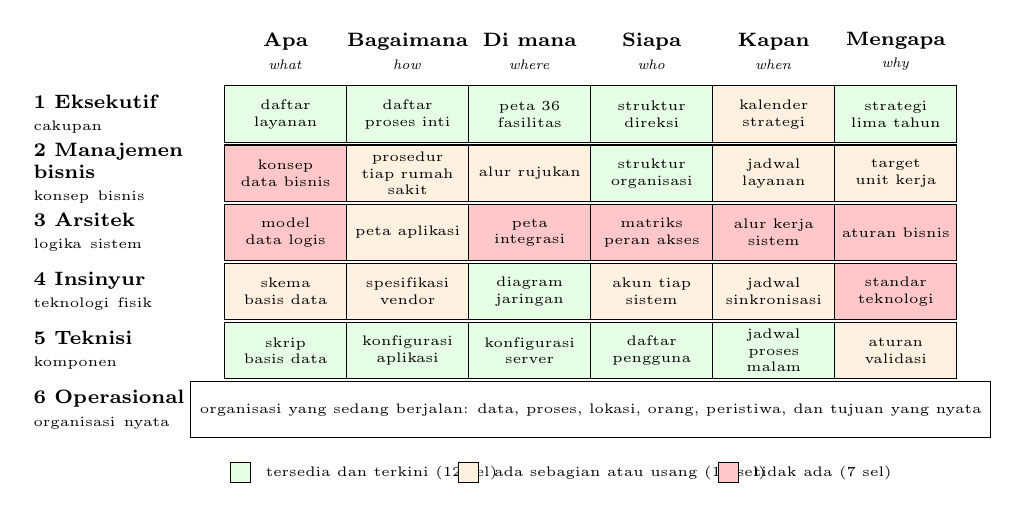
\begin{tikzpicture}[
  font=\scriptsize,
  sel/.style={draw, minimum width=1.55cm, minimum height=0.72cm, text width=1.4cm,
              align=center, font=\tiny, inner sep=1pt},
  kolom/.style={minimum width=1.55cm, minimum height=0.6cm, align=center,
                font=\scriptsize\bfseries, inner sep=1pt},
  baris/.style={minimum width=2.5cm, minimum height=0.72cm, text width=2.35cm,
                align=left, font=\scriptsize\bfseries, inner sep=1pt},
  ada/.style={sel, fill=green!10},
  sebagian/.style={sel, fill=orange!12},
  kosong/.style={sel, fill=red!22}
]
  % Judul kolom: enam kata tanya.
  \node[kolom] at (3.275,0) {Apa\\{\tiny\mdseries\textit{what}}};
  \node[kolom] at (4.825,0) {Bagaimana\\{\tiny\mdseries\textit{how}}};
  \node[kolom] at (6.375,0) {Di mana\\{\tiny\mdseries\textit{where}}};
  \node[kolom] at (7.925,0) {Siapa\\{\tiny\mdseries\textit{who}}};
  \node[kolom] at (9.475,0) {Kapan\\{\tiny\mdseries\textit{when}}};
  \node[kolom] at (11.025,0) {Mengapa\\{\tiny\mdseries\textit{why}}};

  % Baris 1: eksekutif.
  \node[baris] at (1.25,-0.8) {1 Eksekutif\\{\tiny\mdseries cakupan}};
  \node[ada] at (3.275,-0.8) {daftar layanan};
  \node[ada] at (4.825,-0.8) {daftar proses inti};
  \node[ada] at (6.375,-0.8) {peta 36 fasilitas};
  \node[ada] at (7.925,-0.8) {struktur direksi};
  \node[sebagian] at (9.475,-0.8) {kalender strategi};
  \node[ada] at (11.025,-0.8) {strategi lima tahun};

  % Baris 2: manajemen bisnis.
  \node[baris] at (1.25,-1.55) {2 Manajemen bisnis\\{\tiny\mdseries konsep bisnis}};
  \node[kosong] at (3.275,-1.55) {konsep data bisnis};
  \node[sebagian] at (4.825,-1.55) {prosedur tiap rumah sakit};
  \node[sebagian] at (6.375,-1.55) {alur rujukan};
  \node[ada] at (7.925,-1.55) {struktur organisasi};
  \node[sebagian] at (9.475,-1.55) {jadwal layanan};
  \node[sebagian] at (11.025,-1.55) {target unit kerja};

  % Baris 3: arsitek.
  \node[baris] at (1.25,-2.3) {3 Arsitek\\{\tiny\mdseries logika sistem}};
  \node[kosong] at (3.275,-2.3) {model data logis};
  \node[sebagian] at (4.825,-2.3) {peta aplikasi};
  \node[kosong] at (6.375,-2.3) {peta integrasi};
  \node[kosong] at (7.925,-2.3) {matriks peran akses};
  \node[kosong] at (9.475,-2.3) {alur kerja sistem};
  \node[kosong] at (11.025,-2.3) {aturan bisnis};

  % Baris 4: insinyur.
  \node[baris] at (1.25,-3.05) {4 Insinyur\\{\tiny\mdseries teknologi fisik}};
  \node[sebagian] at (3.275,-3.05) {skema basis data};
  \node[sebagian] at (4.825,-3.05) {spesifikasi vendor};
  \node[ada] at (6.375,-3.05) {diagram jaringan};
  \node[sebagian] at (7.925,-3.05) {akun tiap sistem};
  \node[sebagian] at (9.475,-3.05) {jadwal sinkronisasi};
  \node[kosong] at (11.025,-3.05) {standar teknologi};

  % Baris 5: teknisi.
  \node[baris] at (1.25,-3.8) {5 Teknisi\\{\tiny\mdseries komponen}};
  \node[ada] at (3.275,-3.8) {skrip basis data};
  \node[ada] at (4.825,-3.8) {konfigurasi aplikasi};
  \node[ada] at (6.375,-3.8) {konfigurasi server};
  \node[ada] at (7.925,-3.8) {daftar pengguna};
  \node[ada] at (9.475,-3.8) {jadwal proses malam};
  \node[sebagian] at (11.025,-3.8) {aturan validasi};

  % Baris 6: organisasi yang berjalan.
  \node[baris] at (1.25,-4.55) {6 Operasional\\{\tiny\mdseries organisasi nyata}};
  \node[draw, minimum width=9.3cm, minimum height=0.72cm, align=center, font=\tiny,
        fill=white] at (7.15,-4.55)
    {organisasi yang sedang berjalan: data, proses, lokasi, orang, peristiwa, dan tujuan yang nyata};

  % Keterangan warna.
  \node[draw, fill=green!10, minimum size=0.25cm] at (2.7,-5.35) {};
  \node[font=\tiny, anchor=west] at (2.9,-5.35) {tersedia dan terkini (12 sel)};
  \node[draw, fill=orange!12, minimum size=0.25cm] at (5.6,-5.35) {};
  \node[font=\tiny, anchor=west] at (5.8,-5.35) {ada sebagian atau usang (11 sel)};
  \node[draw, fill=red!22, minimum size=0.25cm] at (8.9,-5.35) {};
  \node[font=\tiny, anchor=west] at (9.1,-5.35) {tidak ada (7 sel)};
\end{tikzpicture}

  \caption{Kerangka Zachman sebagai daftar periksa kelengkapan dokumen
           Medikara. Isi sel adalah contoh inventarisasi awal}
  \label{fig:ch02-zachman-medikara}
\end{figure}

\begin{kasus}[title={Kasus Medikara Health: Lemari Arsip yang Kosong di Tengah}]
\setlength{\parskip}{0.4em}
Misalkan tim arsitektur Medikara menginventarisasi dokumen yang sudah ada,
lalu menaruh tiap dokumen di sel Zachman yang sesuai, seperti pada
Gambar \ref{fig:ch02-zachman-medikara}. Dari 30 sel pada baris 1 sampai 5,
sebanyak 12 sel terisi dokumen yang terkini, 11 sel hanya terisi sebagian
atau dokumennya sudah usang, dan 7 sel kosong.

Polanya lebih penting daripada jumlahnya. Baris 1 hampir lengkap, karena
direksi punya strategi, daftar layanan, dan peta fasilitas. Baris 5 juga
hampir lengkap, karena vendor wajib menyerahkan konfigurasi dan skrip, dan
hanya aturan validasi yang tersedia sebagian. Lima dari
tujuh sel kosong berada di baris 3, yaitu logika sistem, baris yang
menghubungkan keputusan direksi dengan konfigurasi teknis. Kekosongan di sel
peta integrasi sejalan dengan biaya integrasi yang tinggi, dan kekosongan di
sel matriks peran akses sejalan dengan temuan audit tentang kontrol akses
yang lemah. Daftar periksa ini tidak berarti ketujuh sel harus segera
diisi. Artinya, setiap keputusan membiarkan sel tetap kosong diambil dengan
sadar, lengkap dengan alasannya.
\end{kasus}

Memakai Zachman berdampingan dengan TOGAF punya dua konsekuensi. Pertama,
kelengkapan menjadi terukur. Tim dapat menyatakan bahwa 7 dari 30 sel masih
kosong, bukan sekadar merasa dokumentasinya kurang. Kedua, muncul godaan
untuk mengisi seluruh 36 sel. Godaan ini perlu dilawan, karena sel yang diisi
tanpa ada pembacanya hanya menambah dokumen yang tidak terpelihara.

\begin{pendalaman}
Bagi mahasiswa berlatar rekayasa perangkat lunak, sel Zachman dapat
dipetakan ke model yang biasa dibuat tim pengembang. Tabel
\ref{tab:ch02-zachman-rpl} memuat pemetaan yang lazim untuk baris 3 sampai
5. Pemetaan ini tidak resmi, tetapi memperlihatkan bahwa sebagian besar
model rekayasa perangkat lunak menumpuk di kolom apa, bagaimana, dan di mana.

\begin{center}
  \captionof{table}{Pemetaan sel Zachman ke model rekayasa perangkat lunak}
  \label{tab:ch02-zachman-rpl}
  {\footnotesize
  \begin{tabularx}{\linewidth}{>{\raggedright\arraybackslash}p{3.0cm}
                               >{\raggedright\arraybackslash}X}
    \hline
    \textbf{Sel Zachman} & \textbf{Model yang lazim} \\
    \hline
    Baris 3, apa & Model data logis, diagram entitas dan relasi \\
    \hline
    Baris 3, bagaimana & Diagram komponen, diagram aktivitas \\
    \hline
    Baris 3, siapa & Diagram \textit{use case}, matriks peran dan hak akses \\
    \hline
    Baris 3, kapan & Diagram \textit{sequence}, diagram status \\
    \hline
    Baris 4, apa & Skema basis data fisik \\
    \hline
    Baris 4, di mana & Diagram \textit{deployment} \\
    \hline
    Baris 4, mengapa & Catatan keputusan arsitektur, standar teknologi \\
    \hline
    Baris 5, semua kolom & Kode sumber, berkas konfigurasi, skrip infrastruktur \\
    \hline
  \end{tabularx}}
\end{center}

Dugaan yang layak diuji: kolom siapa, kapan, dan mengapa paling sering
kosong, karena aturan bisnis dan alasan keputusan jarang ditulis di luar
kode. Dugaan ini dibuktikan dengan memeriksa repositori proyek nyata memakai
\berkas{sources/chapter02/daftar-periksa-zachman.md}.
\end{pendalaman}

\section{Arsitektur SPBE}

TOGAF dan Zachman bersifat sukarela. Instansi pemerintah di Indonesia tidak
punya pilihan itu, karena kerangkanya ditetapkan peraturan. Peraturan
Presiden (Perpres) Nomor 95 Tahun 2018 tentang SPBE mendefinisikan Arsitektur
SPBE sebagai kerangka dasar yang mendeskripsikan integrasi proses bisnis,
data dan informasi, infrastruktur SPBE, aplikasi SPBE, dan keamanan SPBE
untuk menghasilkan layanan SPBE yang terintegrasi (Pasal 1 angka 6)
\cite{perpres95-2018}. Arsitektur SPBE terdiri atas tiga tingkat: nasional,
instansi pusat, dan pemerintah daerah (Pasal 6). Arsitektur SPBE Nasional
memuat referensi arsitektur, yaitu komponen dasar baku yang menjadi acuan,
dan domain arsitektur, yaitu substansinya (Pasal 7 ayat (2)).

Domain arsitektur itu ada enam: proses bisnis, data dan informasi,
infrastruktur SPBE, aplikasi SPBE, keamanan SPBE, dan layanan SPBE (Pasal 7
ayat (4)). Setiap tingkat disusun untuk jangka waktu lima tahun dan ditinjau
pada paruh waktu dan tahun terakhir pelaksanaan (Pasal 8, Pasal 11, dan
Pasal 12). Tingkat nasional disusun berdasarkan Rencana Induk SPBE Nasional
dan Rencana Pembangunan Jangka Menengah Nasional (Pasal 9 ayat (1)), sedangkan
tingkat pemerintah daerah berpedoman pada Arsitektur SPBE Nasional dan
Rencana Pembangunan Jangka Menengah Daerah (Pasal 12 ayat (1)).

Analoginya seperti tata ruang wilayah. Ada rencana tata ruang nasional,
provinsi, dan kabupaten, dan rencana yang lebih rendah wajib selaras dengan
yang di atasnya. Setiap gedung tetap punya gambar sendiri, tetapi gambar itu
tidak boleh melanggar peruntukan zonanya. Arsitektur SPBE instansi adalah
gambar gedungnya, dan Arsitektur SPBE Nasional adalah peta zonanya.

Perpres Nomor 132 Tahun 2022 menetapkan Arsitektur SPBE Nasional untuk
periode 2020 sampai 2024 \cite{perpres132-2022}. Perpres Nomor 82 Tahun 2023
menetapkan Aplikasi SPBE Prioritas yang mengutamakan integrasi dan
interoperabilitas, antara lain untuk layanan pendidikan, kesehatan, bantuan
sosial, dan administrasi kependudukan, serta menugaskan Perum Peruri untuk
menyelenggarakannya \cite{perpres82-2023}. Perpres Nomor 83 Tahun 2025
membentuk Komite Percepatan Transformasi Digital Pemerintah, dengan salah
satu wakil ketua yang membidangi tata kelola pemerintah digital, termasuk
arsitektur pemerintah digital \cite{perpres83-2025}. Evaluasinya kini diatur
Peraturan Menteri PANRB (Pendayagunaan Aparatur Negara dan Reformasi
Birokrasi) Nomor 8 Tahun 2026 tentang Evaluasi Kinerja Pemerintah Digital
\cite{permenpanrb8-2026}.

Status per 30 Oktober 2026 perlu dicatat dengan hati-hati. Perpres 95/2018
masih berlaku, dan revisinya menjadi Perpres tentang Pemerintah Digital masih
disusun. Arsitektur SPBE Nasional yang ditetapkan tetap untuk periode 2020
sampai 2024, dan penggantinya untuk periode berikutnya belum ditemukan. Tim
yang memakai instansi pemerintah perlu memeriksa ulang status ini di basis
data peraturan resmi, misalnya \url{https://peraturan.bpk.go.id}.

Dua contoh penerapannya:

\begin{enumerate}
  \item Sebuah pemerintah kabupaten menyusun Arsitektur SPBE Pemerintah
        Daerah untuk 2026 sampai 2030, mengikuti Rencana Pembangunan Jangka
        Menengah Daerahnya. Dokumen itu ditinjau pada paruh waktu dan pada
        tahun terakhir. Bila Arsitektur SPBE Nasional berubah di tengah
        periode, perubahan itu menjadi salah satu dasar peninjauan (Pasal 12
        ayat (6)).
  \item Misalkan kabupaten yang sama punya satu rumah sakit umum daerah dan
        25 puskesmas. Aplikasi pendaftaran pasien di 26 fasilitas itu masuk
        domain aplikasi SPBE, sedangkan layanan pendaftaran daring yang
        dipakai warga masuk domain layanan SPBE.
\end{enumerate}

\subsection*{Enam domain SPBE dan empat domain TOGAF}

TOGAF mengenal empat domain arsitektur: bisnis, data, aplikasi, dan
teknologi \cite{togaf10}. Gambar \ref{fig:ch02-domain-spbe-togaf} memetakan
keenam domain SPBE ke keempat domain itu. Empat domain punya padanan
langsung, dan dua domain tidak punya.

\begin{figure}[!htb]
  \centering
  \begin{tikzpicture}[
  font=\scriptsize,
  dom/.style={draw, rounded corners, minimum height=0.7cm, minimum width=3.4cm,
              align=center, font=\scriptsize},
  panah/.style={-{Stealth[length=2mm]}, thick},
  sebagian/.style={-{Stealth[length=2mm]}, thick, dashed}
]
  \node[font=\scriptsize\bfseries] at (0,3.3) {Arsitektur SPBE: enam domain};
  \node[font=\scriptsize\bfseries] at (7.8,3.3) {TOGAF: empat domain};

  \node[dom, fill=blue!8] (pb) at (0,2.5) {Proses Bisnis};
  \node[dom, fill=orange!12] (lay) at (0,1.5) {Layanan SPBE};
  \node[dom, fill=blue!8] (dat) at (0,0.5) {Data dan Informasi};
  \node[dom, fill=blue!8] (apl) at (0,-0.5) {Aplikasi SPBE};
  \node[dom, fill=blue!8] (inf) at (0,-1.5) {Infrastruktur SPBE};
  \node[dom, fill=orange!12] (kea) at (0,-2.5) {Keamanan SPBE};

  \node[dom, fill=praditagreen!15] (bis) at (7.8,2.0) {Arsitektur Bisnis};
  \node[dom, fill=praditagreen!15] (tdat) at (7.8,0.5) {Arsitektur Data};
  \node[dom, fill=praditagreen!15] (tapl) at (7.8,-0.5) {Arsitektur Aplikasi};
  \node[dom, fill=praditagreen!15] (tek) at (7.8,-1.5) {Arsitektur Teknologi};
  \node[dom, fill=green!10, dashed] (lintas) at (7.8,-2.7)
    {\textit{Concern} lintas domain\\{\tiny\textit{Series Guide} keamanan}};

  \draw[panah] (pb.east) -- (bis.west);
  \draw[sebagian] (lay.east) -- node[font=\tiny, above, sloped] {layanan bisnis} (bis.west);
  \draw[sebagian] (lay.east) -- node[font=\tiny, below, sloped, pos=0.62] {layanan aplikasi} (tapl.west);
  \draw[panah] (dat.east) -- (tdat.west);
  \draw[panah] (apl.east) -- (tapl.west);
  \draw[panah] (inf.east) -- (tek.west);
  \draw[sebagian] (kea.east) -- (lintas.west);

  \node[font=\tiny, anchor=west] at (-1.7,-3.35) {garis utuh: padanan langsung};
  \node[font=\tiny, anchor=west] at (2.0,-3.35) {garis putus: padanan sebagian atau lintas domain};
\end{tikzpicture}

  \caption{Pemetaan enam domain Arsitektur SPBE ke empat domain arsitektur
           TOGAF}
  \label{fig:ch02-domain-spbe-togaf}
\end{figure}

Domain layanan SPBE berdiri sendiri karena Perpres 95/2018 mendefinisikan
layanan SPBE sebagai keluaran yang dihasilkan satu atau beberapa fungsi
aplikasi SPBE dan memiliki nilai manfaat (Pasal 1 angka 4). Di TOGAF, isi itu
terbagi dua: layanan yang dirasakan warga masuk arsitektur bisnis, sedangkan
fungsi aplikasi yang menghasilkannya masuk arsitektur aplikasi. Domain
keamanan SPBE juga berdiri sendiri, sedangkan TOGAF memperlakukan keamanan
sebagai \textit{concern} yang melintasi semua domain dan membahasnya dalam
\textit{Series Guide} tersendiri \cite{c02-togaf-pocket}. Tabel
\ref{tab:ch02-domain-spbe} melengkapi pemetaan itu dengan koordinator tiap
domain di tingkat nasional.

\begin{table}[!htb]
  \centering
  \caption{Domain Arsitektur SPBE, koordinatornya menurut Pasal 9 ayat (3)
           Perpres 95/2018, dan padanannya di TOGAF}
  \label{tab:ch02-domain-spbe}
  {\footnotesize
  \begin{tabularx}{\textwidth}{>{\raggedright\arraybackslash}p{2.6cm}
                               >{\raggedright\arraybackslash}X
                               >{\raggedright\arraybackslash}X}
    \hline
    \textbf{Domain SPBE} & \textbf{Koordinator nasional} & \textbf{Padanan TOGAF} \\
    \hline
    Proses bisnis & Menteri bidang aparatur negara & Arsitektur bisnis, langsung \\
    \hline
    Layanan SPBE & Menteri bidang aparatur negara & Sebagian di arsitektur bisnis, sebagian di arsitektur aplikasi \\
    \hline
    Data dan informasi & Menteri bidang perencanaan pembangunan nasional & Arsitektur data, langsung \\
    \hline
    Aplikasi SPBE & Menteri bidang komunikasi dan informatika & Arsitektur aplikasi, langsung \\
    \hline
    Infrastruktur SPBE & Menteri bidang komunikasi dan informatika & Arsitektur teknologi, langsung \\
    \hline
    Keamanan SPBE & Kepala lembaga bidang keamanan siber & Tidak ada domain tersendiri, ditangani sebagai \textit{concern} lintas domain \\
    \hline
  \end{tabularx}}
\end{table}

Perbedaan jumlah domain ini punya dua konsekuensi bagi tim yang memakai ADM
di instansi pemerintah. Pertama, artefak layanan dan keamanan harus
dijadwalkan secara eksplisit di fase B sampai D, karena ADM tidak punya fase
khusus untuk keduanya. Kedua, koordinatornya berbeda. Keamanan dikoordinasi
lembaga di bidang keamanan siber, bukan oleh kementerian yang membina
aplikasi, sehingga tanpa pemetaan yang jelas dua instansi pembina dapat
menerima dokumen yang saling tumpang tindih.

\begin{kasus}[title={Kasus Medikara Health: Mengapa Perusahaan Swasta Membaca Arsitektur Pemerintah}]
Medikara adalah perusahaan swasta, sehingga tidak wajib menyusun Arsitektur
SPBE. Namun Perpres 95/2018 menyebut pelaku usaha sebagai salah satu Pengguna
SPBE (Pasal 1 angka 26), dan Medikara memang memakai layanan pemerintah
setiap hari. Data layanan dikirim ke SATUSEHAT milik Kementerian Kesehatan
dengan standar HL7 FHIR, dan klaim pasien jaminan kesehatan dikirim ke BPJS
Kesehatan. Layanan kesehatan juga termasuk bidang Aplikasi SPBE Prioritas
dalam Perpres 82/2023. Akibatnya, perubahan di sisi pemerintah merambat ke
Medikara. Perubahan format data di SATUSEHAT mengubah antarmuka kelima SIMRS,
dan perubahan aturan klaim mengubah proses di loket. Karena itu arsitek
Medikara memantau perkembangan Arsitektur SPBE dan Peraturan Menteri
Kesehatan Nomor 24 Tahun 2022 tentang Rekam Medis \cite{permenkes24-2022},
sama seperti bagian keuangan memantau peraturan perpajakan. Rincian
integrasinya dibahas di IT40613.
\end{kasus}

\section{Menyesuaikan Kerangka untuk Organisasi}

Pertanyaan berikutnya: apakah seluruh isi TOGAF harus dikerjakan? Jawabannya
tidak, dan TOGAF sendiri tidak memintanya. Fase \textit{Preliminary}
menghasilkan kerangka yang disesuaikan (\textit{Tailored Architecture
Framework}), yaitu keputusan tertulis tentang fase, teknik, dan artefak yang
benar-benar dipakai organisasi itu \cite{c02-togaf-pocket}. Penyesuaian
mempertimbangkan ukuran organisasi, jumlah arsitek, kematangan praktik yang
sudah ada, dan regulasi yang mengikat.

Bukti empiris mendukung langkah ini. Kotusev meneliti artefak EA di 27
organisasi dan menemukan 24 artefak umum yang terbukti berguna dalam praktik
\cite{kotusev2019}. Temuannya juga mempertanyakan pandangan bahwa EA cukup
dipahami sebagai empat domain arsitektur, atau sebagai rangkaian kondisi saat
ini, kondisi target, dan peta jalan. Dalam bukunya, Kotusev mengelompokkan
artefak menjadi enam jenis: \textit{considerations} seperti prinsip,
\textit{standards} seperti standar teknologi, \textit{visions} seperti
\textit{capability map} dan peta jalan, \textit{landscapes} seperti diagram
lanskap, \textit{outlines} seperti gambaran ringkas solusi, dan
\textit{designs} seperti rancangan rinci solusi \cite{kotusev2021}. Organisasi
memakai campuran beberapa jenis, bukan seluruh daftar artefak sebuah
kerangka.

Analoginya seperti memasak dari buku resep untuk 50 porsi, padahal yang
makan hanya delapan orang. Takaran bahan dikecilkan, dan hiasan yang tidak
perlu dilewati. Satu hal tidak boleh dilewati, yaitu langkah yang menjaga
makanan aman dimakan. Pada kerangka arsitektur, langkah itu adalah yang
menjaga keputusan dapat ditelusuri: siapa pemangku kepentingannya, apa
\textit{concern}-nya, dan artefak mana yang menjawabnya.

Dua contoh penyesuaian:

\begin{enumerate}
  \item Misalkan tim arsitektur Medikara hanya tiga orang dan harus melayani
        36 fasilitas. Tim memilih 12 artefak untuk cetak biru 2026 sampai
        2030. Model data logis hanya dibuat untuk entitas Pasien dan
        Kunjungan, karena keduanya inti strategi ``Satu Pasien, Satu Rekam
        Medis''.
  \item Misalkan sebuah pemerintah kabupaten hanya punya dua pegawai yang
        memahami arsitektur. Kabupaten itu tetap wajib memuat enam domain
        SPBE, tetapi domain layanan dan aplikasi dirinci lebih dahulu, karena
        keduanya paling dekat dengan warga yang dilayani.
\end{enumerate}

Tabel \ref{tab:ch02-artefak-minimum} memuat artefak minimum cetak biru
\textit{capstone} hasil penyesuaian untuk semester ini. Tim yang memakai
organisasi sendiri boleh mengubahnya, asalkan alasannya ditulis di
\textit{Statement of Architecture Work}.

\begin{table}[!htb]
  \centering
  \caption{Artefak minimum cetak biru \textit{capstone}, fase ADM asalnya,
           dan pertemuan yang menghasilkannya}
  \label{tab:ch02-artefak-minimum}
  {\footnotesize
  \begin{tabularx}{\textwidth}{>{\raggedright\arraybackslash}X
                               >{\raggedright\arraybackslash}p{1.9cm}
                               >{\raggedright\arraybackslash}p{2.9cm}
                               >{\raggedright\arraybackslash}p{1.6cm}}
    \hline
    \textbf{Artefak} & \textbf{Fase ADM} & \textbf{Bentuk} & \textbf{Pertemuan} \\
    \hline
    Peta pemangku kepentingan dan \textit{concern} & A & Matriks dan diagram & 2 \\
    \hline
    \textit{Statement of Architecture Work} & A & \textit{Deliverable} & 2 \\
    \hline
    Prinsip arsitektur & \textit{Preliminary} & Katalog & 3 \\
    \hline
    Visi arsitektur & A & \textit{Deliverable} & 3 \\
    \hline
    Model ArchiMate berlapis & B sampai D & Diagram & 4 \\
    \hline
    \textit{Capability map} dan \textit{heatmap} & B & Diagram & 5, 8 \\
    \hline
    Matriks CRUD (\textit{Create, Read, Update, Delete}) & C & Matriks & 6 \\
    \hline
    Katalog aplikasi dan diagram integrasi & C, D & Katalog dan diagram & 7, 9 \\
    \hline
    Catatan keputusan arsitektur & D & Dokumen singkat & 10 \\
    \hline
    Matriks gap dan paket kerja & E & Matriks & 11 \\
    \hline
    Peta jalan dan rencana migrasi & E, F & Diagram dan \textit{deliverable} & 12 \\
    \hline
    Rancangan tata kelola arsitektur & G, H & \textit{Deliverable} & 14 \\
    \hline
  \end{tabularx}}
\end{table}

Penyesuaian juga punya batas. Kerangka adalah alat, bukan tujuan, tetapi alat
yang dipotong terlalu banyak kehilangan gunanya. Dua tanda bahwa penyesuaian
sudah kebablasan: ada pemain kunci yang \textit{concern}-nya tidak dijawab
artefak mana pun, atau ada keputusan besar yang tidak dapat ditelusuri ke
prinsip dan kebutuhan. Bila salah satu tanda itu muncul, artefak yang
dibuang perlu dikembalikan.

\section{Aktivitas: Peta Pemangku Kepentingan dan Ruang Lingkup Arsitektur}

\subsection*{Tujuan dan pembagian peran}

Aktivitas ini menjawab dua pertanyaan sebelum tim mulai menggambar: siapa
yang berkepentingan atas cetak biru, dan sampai di mana batas pekerjaan
arsitekturnya. Tim bekerja dengan organisasi yang dipilih pada Bab 1, atau
dengan Medikara Health bila tidak punya akses ke organisasi nyata.

\begin{itemize}
  \item \textbf{Analis bisnis} memimpin identifikasi pemangku kepentingan dan
        \textit{concern} bisnisnya, lewat bagan organisasi, wawancara
        singkat, dan dokumen strategi.
  \item \textbf{Analis teknologi} melengkapi \textit{concern} teknis dan
        regulasi, termasuk vendor, regulator, dan sistem pemerintah yang
        terhubung.
  \item \textbf{Pemodel} memilih fase ADM dan artefak minimum, berangkat dari
        Tabel \ref{tab:ch02-artefak-minimum}.
  \item \textbf{Koordinator} merangkum ruang lingkup dalam \textit{Statement
        of Architecture Work} dan menjaga konsistensinya dengan piagam tim.
\end{itemize}

\subsection*{Langkah kerja}

\begin{enumerate}
  \item Daftarkan minimal 10 kelompok pemangku kepentingan dengan templat
        \berkas{sources/chapter02/templat-peta-pemangku-kepentingan.md}.
        Tim Medikara dapat berangkat dari
        \berkas{sources/chapter02/pemangku-kepentingan-medikara.csv}.
  \item Beri nilai kekuasaan dan kepentingan tiap kelompok dengan skala 1
        sampai 5, lengkap dengan alasan satu kalimat. Nilai 3 ke atas
        dianggap tinggi. Tempatkan hasilnya di matriks seperti
        Gambar \ref{fig:ch02-matriks-pemangku}.
  \item Tulis satu sampai tiga \textit{concern} tiap kelompok sebagai
        pertanyaan yang dapat dijawab dengan data, lalu tandai
        \textit{concern} yang berasal dari regulasi.
  \item Untuk tiap \textit{concern} pemain kunci, tentukan \textit{view} yang
        menjawabnya beserta bentuknya: katalog, matriks, atau diagram.
  \item Tetapkan ruang lingkup: unit organisasi, horizon waktu, domain
        arsitektur, dan batasan yang disepakati.
  \item Pilih fase ADM dan artefak minimum, lalu tulis alasan untuk setiap
        artefak yang ditambah atau dibuang dari
        Tabel \ref{tab:ch02-artefak-minimum}.
  \item Bila organisasinya instansi pemerintah, petakan domain TOGAF ke enam
        domain SPBE dengan
        \berkas{sources/chapter02/pemetaan-domain-togaf-spbe.md}.
  \item Rangkai seluruh hasil dalam \textit{Statement of Architecture Work}
        dua sampai tiga halaman memakai
        \berkas{sources/chapter02/templat-statement-of-architecture-work.md}.
\end{enumerate}

Tabel \ref{tab:ch02-sow-medikara} memperlihatkan contoh ringkas
\textit{Statement of Architecture Work} untuk Medikara. Komponennya mengikuti
TOGAF: latar belakang, ruang lingkup, peran, kriteria penerimaan, jadwal, dan
persetujuan \cite{c02-togaf-pocket}.

\begin{table}[!htb]
  \centering
  \caption{Contoh ringkas \textit{Statement of Architecture Work} Medikara}
  \label{tab:ch02-sow-medikara}
  {\footnotesize
  \begin{tabularx}{\textwidth}{>{\raggedright\arraybackslash}p{2.6cm}
                               >{\raggedright\arraybackslash}X}
    \hline
    \textbf{Komponen} & \textbf{Isi untuk Medikara} \\
    \hline
    Latar belakang & Strategi ``Satu Pasien, Satu Rekam Medis''; insiden kebocoran data lewat vendor pada 2025; temuan audit kontrol akses; antrean panjang; biaya integrasi tinggi \\
    \hline
    Unit organisasi & 5 rumah sakit, 18 klinik pratama, 1 laboratorium rujukan, 12 apotek, dan kantor pusat \\
    \hline
    Horizon waktu & Kondisi saat ini per 2026, kondisi target 2030, dengan arsitektur transisi di antaranya \\
    \hline
    Domain & Bisnis, data, aplikasi, dan teknologi; keamanan dan kepatuhan sebagai \textit{concern} lintas domain \\
    \hline
    Batasan & Misalkan ERP keuangan tidak diganti pada siklus ini; hanya antarmukanya yang ditinjau \\
    \hline
    Peran & Sponsor: Direktur Utama; pemilik arsitektur: kepala TI; tim: koordinator, analis bisnis, analis teknologi, pemodel \\
    \hline
    Kriteria penerimaan & Setiap \textit{concern} pemain kunci dijawab minimal satu \textit{view}; seluruh artefak minimum tersedia pada tonggak C1 sampai C4 \\
    \hline
    Jadwal & C1 Pertemuan 3, C2 menjelang UTS, C3 Pertemuan 11, C4 menjelang UAS (Ujian Akhir Semester) \\
    \hline
    Persetujuan & Ditandatangani sponsor dan pemilik arsitektur \\
    \hline
  \end{tabularx}}
\end{table}

\subsection*{Luaran, tonggak, dan penilaian}

Luarannya dua: peta pemangku kepentingan lengkap dengan \textit{concern} dan
\textit{view}-nya, serta \textit{Statement of Architecture Work}. Keduanya
masuk tonggak C1 bersama piagam tim, profil organisasi, dan glosarium dari
Bab 1, lalu dilengkapi visi arsitektur pada Bab 3. Peta pemangku kepentingan
juga dipakai tiga mata kuliah lain: IT40613 untuk mengenali calon mitra
ekosistem, IT40713 untuk mengenali pemilik sistem yang akan dimigrasikan, dan
IT40813 untuk menyusun struktur tanggung jawab tata kelola. Tabel
\ref{tab:ch02-kriteria} memuat kriteria penilaian yang dipakai saat tatap
muka hari Sabtu. Daftar lengkap berkas pendukung ada di
\berkas{sources/chapter02/README.md}.

\begin{table}[!htb]
  \centering
  \caption{Kriteria penilaian Aktivitas Bab 2}
  \label{tab:ch02-kriteria}
  {\footnotesize
  \begin{tabularx}{\textwidth}{>{\raggedright\arraybackslash}p{3.6cm}
                               >{\raggedright\arraybackslash}p{1.2cm}
                               >{\raggedright\arraybackslash}X}
    \hline
    \textbf{Kriteria} & \textbf{Bobot} & \textbf{Ciri hasil yang baik} \\
    \hline
    Kelengkapan pemangku kepentingan & 25\% & Pihak luar dan regulator tercatat; penempatan di matriks disertai alasan \\
    \hline
    Ketajaman \textit{concern} & 25\% & Ditulis sebagai pertanyaan yang dapat dijawab dengan data \\
    \hline
    Kejelasan ruang lingkup & 30\% & Unit, horizon waktu, domain, dan batasan tertulis eksplisit \\
    \hline
    Kesesuaian artefak dan fase & 20\% & Setiap artefak yang ditambah atau dibuang punya alasan \\
    \hline
  \end{tabularx}}
\end{table}

\textit{Pendalaman teknis (opsional):} mahasiswa berlatar ilmu komputer,
rekayasa perangkat lunak, atau teknologi informasi memetakan sel Zachman ke
model yang lazim dibuat tim pengembang, seperti pada kotak pendalaman seksi
Zachman, lalu menilai sel mana yang paling sering kosong di satu proyek nyata
memakai \berkas{sources/chapter02/daftar-periksa-zachman.md}. Hasilnya tidak
masuk penilaian tonggak, tetapi menjadi bahan diskusi dengan anggota tim
berlatar bisnis.

\section{Ringkasan}

Dokumen arsitektur yang tidak dapat dibandingkan biasanya bukan dokumen yang
salah, melainkan dokumen yang tidak menyebut pembaca dan pertanyaannya.
ISO/IEC/IEEE 42010:2022 memberi kosakata untuk menutup celah itu: pemangku
kepentingan memiliki \textit{concern}, \textit{viewpoint} membingkai
\textit{concern} dan mengatur pembuatan \textit{view}, dan \textit{view}
menjawab \textit{concern}. Matriks kekuasaan dan kepentingan menentukan
\textit{concern} siapa yang didahulukan, dan untuk Medikara hasilnya sepuluh
kelompok, dari direksi sampai vendor.

TOGAF Standard edisi ke-10 terbagi menjadi \textit{Fundamental Content} yang
jarang berubah dan \textit{Series Guides} yang menyesuaikannya dengan topik
tertentu. Pembaruan 2025 memasukkan \textit{Technical Corrigendum} 1 tanpa
mengubah susunan itu. Intinya adalah ADM, siklus berisi \textit{Preliminary},
fase A sampai H, dan Manajemen Kebutuhan di tengah. Tiga istilahnya perlu
dibedakan dengan tegas: \textit{deliverable} disetujui secara formal, artefak
berbentuk katalog, matriks, atau diagram, dan \textit{building block} adalah
komponen yang dapat dipakai ulang.

Zachman Framework bukan pesaing ADM. Zachman adalah ontologi berupa matriks
enam kata tanya dan enam sudut pandang, sedangkan ADM adalah metode. ADM
menghasilkan artefak, dan Zachman memeriksa kelengkapannya. Pada contoh
inventarisasi Medikara, 7 dari 30 sel kosong, dan lima di antaranya berada di
baris logika sistem, yaitu baris yang menghubungkan keputusan direksi dengan
konfigurasi teknis.

Arsitektur SPBE diwajibkan bagi instansi pemerintah lewat Perpres 95/2018,
dengan tiga tingkat, jangka waktu lima tahun, dan enam domain. Empat
domainnya punya padanan langsung di TOGAF, sedangkan layanan dan keamanan
harus ditangani secara eksplisit. Medikara tidak wajib menyusun Arsitektur
SPBE, tetapi tetap perlu membacanya, karena SATUSEHAT dan BPJS Kesehatan
membatasi pilihan arsitekturnya.

Kerangka kerja adalah alat, bukan tujuan. TOGAF sendiri meminta penyesuaian
lewat fase \textit{Preliminary}, dan penelitian Kotusev di 27 organisasi
menunjukkan bahwa praktik nyata memakai campuran artefak, bukan seluruh
daftar. Penyesuaian yang baik membuang artefak tanpa pembaca, tetapi tetap
menjaga setiap keputusan dapat ditelusuri ke pemangku kepentingan dan
\textit{concern}-nya. Karena itulah Aktivitas bab ini dimulai dari peta
pemangku kepentingan, bukan dari diagram.

\section{Latihan}

Ketiga latihan dikerjakan secara mandiri tanpa perangkat lunak khusus.
Berkas pendukungnya tersedia di \berkas{sources/chapter02/}. Hasil tiap
mahasiswa boleh berbeda. Yang dinilai adalah penalaran dan perbandingannya,
bukan kecocokan dengan contoh.

\subsection*{Latihan 1: Concern Direktur Keuangan dan Kepala TI}

Latihan ini membuktikan bahwa satu proyek yang sama menuntut \textit{view}
yang berbeda bagi pembaca yang berbeda. Misalkan proyek yang dinilai adalah
pembangunan layanan identitas pasien tunggal untuk 36 fasilitas Medikara.

\begin{enumerate}
  \item Baca ulang Gambar \ref{fig:ch02-konsep-42010} dan
        Tabel \ref{tab:ch02-concern-medikara}.
  \item Tulis dua \textit{concern} Direktur Keuangan dan dua \textit{concern}
        kepala TI atas proyek itu, masing-masing sebagai pertanyaan yang
        dapat dijawab dengan data.
  \item Tentukan \textit{view} untuk tiap \textit{concern}: isinya, bentuknya
        (katalog, matriks, atau diagram), dan sumber datanya.
  \item Tandai \textit{concern} yang dimiliki keduanya, lalu putuskan apakah
        satu \textit{view} cukup untuk keduanya.
  \item Isi Tabel \ref{tab:ch02-lat1-hasil}. Tabel \ref{tab:ch02-lat1-contoh}
        memperlihatkan contoh yang sudah terisi.
\end{enumerate}

\begin{table}[!htb]
  \centering
  \caption{Contoh hasil Latihan 1 yang sudah terisi}
  \label{tab:ch02-lat1-contoh}
  {\footnotesize
  \begin{tabularx}{\textwidth}{>{\raggedright\arraybackslash}p{2.0cm}
                               >{\raggedright\arraybackslash}X
                               >{\raggedright\arraybackslash}p{2.8cm}
                               >{\raggedright\arraybackslash}p{2.8cm}}
    \hline
    \textbf{Pemangku} & \textbf{\textit{Concern}} & \textbf{\textit{View}} & \textbf{Bentuk dan sumber} \\
    \hline
    Direktur Keuangan & Berapa total biaya proyek sampai 2030, dan kapan manfaatnya mulai terlihat? & Ringkasan biaya dan manfaat per tahun & Tabel; penawaran vendor dan biaya integrasi saat ini \\
    \hline
    Kepala TI & Berapa antarmuka \textit{point-to-point} yang hilang setelah proyek selesai? & Integrasi sebelum dan sesudah proyek & Diagram; katalog antarmuka \\
    \hline
  \end{tabularx}}
\end{table}

\begin{table}[!htb]
  \centering
  \caption{Lembar isian Latihan 1}
  \label{tab:ch02-lat1-hasil}
  {\footnotesize
  \begin{tabularx}{\textwidth}{>{\raggedright\arraybackslash}p{2.0cm}
                               >{\raggedright\arraybackslash}X
                               >{\raggedright\arraybackslash}p{2.8cm}
                               >{\raggedright\arraybackslash}p{2.8cm}}
    \hline
    \textbf{Pemangku} & \textbf{\textit{Concern}} & \textbf{\textit{View}} & \textbf{Bentuk dan sumber} \\
    \hline
    Direktur Keuangan & \dots & \dots & \dots \\
    \hline
    Direktur Keuangan & \dots & \dots & \dots \\
    \hline
    Kepala TI & \dots & \dots & \dots \\
    \hline
    Kepala TI & \dots & \dots & \dots \\
    \hline
  \end{tabularx}}
\end{table}

Jawab dua pertanyaan berikut berdasarkan tabel yang sudah diisi. Pertama,
\textit{concern} mana yang belum dapat dijawab dengan data yang tersedia di
Medikara saat ini, dan data apa yang kurang? Kedua, bila satu \textit{view}
dipakai untuk melayani kedua pemangku kepentingan, informasi apa yang
dikorbankan bagi masing-masing?

\subsection*{Latihan 2: Ontologi dan Metode}

Latihan ini membuktikan bahwa Zachman dan ADM menjawab pertanyaan yang
berbeda, sehingga keduanya dapat dipakai bersama tanpa saling menggantikan.

\begin{enumerate}
  \item Pilih enam artefak dari Tabel \ref{tab:ch02-artefak-minimum}.
  \item Tentukan sel Zachman tiap artefak, yaitu baris dan kolomnya, memakai
        \berkas{sources/chapter02/daftar-periksa-zachman.md}. Satu artefak
        boleh menempati lebih dari satu sel.
  \item Tentukan fase ADM tempat artefak itu dibuat, memakai
        Tabel \ref{tab:ch02-fase-adm}.
  \item Catat sel penting yang tidak diisi artefak mana pun, lalu putuskan
        apakah sel itu perlu diisi.
  \item Isi Tabel \ref{tab:ch02-lat2-hasil}. Tabel \ref{tab:ch02-lat2-contoh}
        memperlihatkan contoh yang sudah terisi.
\end{enumerate}

\begin{table}[!htb]
  \centering
  \caption{Contoh hasil Latihan 2 yang sudah terisi}
  \label{tab:ch02-lat2-contoh}
  {\footnotesize
  \begin{tabularx}{\textwidth}{>{\raggedright\arraybackslash}p{2.8cm}
                               >{\raggedright\arraybackslash}p{3.2cm}
                               >{\raggedright\arraybackslash}p{1.0cm}
                               >{\raggedright\arraybackslash}X}
    \hline
    \textbf{Artefak} & \textbf{Sel Zachman} & \textbf{Fase} & \textbf{Catatan} \\
    \hline
    Matriks CRUD & Baris 3, kolom apa dan bagaimana & C & Satu artefak menghubungkan dua kolom \\
    \hline
    Peta pemangku kepentingan & Baris 1 dan 2, kolom siapa & A & Kolom siapa terisi lebih awal daripada kolom lain \\
    \hline
  \end{tabularx}}
\end{table}

\begin{table}[!htb]
  \centering
  \caption{Lembar isian Latihan 2}
  \label{tab:ch02-lat2-hasil}
  {\footnotesize
  \begin{tabularx}{\textwidth}{>{\raggedright\arraybackslash}p{2.8cm}
                               >{\raggedright\arraybackslash}p{3.2cm}
                               >{\raggedright\arraybackslash}p{1.0cm}
                               >{\raggedright\arraybackslash}X}
    \hline
    \textbf{Artefak} & \textbf{Sel Zachman} & \textbf{Fase} & \textbf{Catatan} \\
    \hline
    \dots & \dots & \dots & \dots \\
    \hline
    \dots & \dots & \dots & \dots \\
    \hline
    \dots & \dots & \dots & \dots \\
    \hline
    \dots & \dots & \dots & \dots \\
    \hline
    \dots & \dots & \dots & \dots \\
    \hline
    \dots & \dots & \dots & \dots \\
    \hline
  \end{tabularx}}
\end{table}

Jawab tiga pertanyaan berikut berdasarkan tabel yang sudah diisi. Pertama,
kolom tabel mana yang menyatakan jenis isi sebuah artefak, dan kolom mana yang
menyatakan kapan artefak itu dibuat? Jelaskan hubungannya dengan sebutan
ontologi bagi Zachman dan metode bagi ADM. Kedua, apa akibatnya bila tim
memaksa mengisi seluruh 36 sel? Ketiga, sel kosong mana yang paling berisiko
bagi strategi ``Satu Pasien, Satu Rekam Medis'', dan mengapa?

\subsection*{Latihan 3: Enam Domain SPBE dan Empat Domain TOGAF}

Latihan ini membuktikan bahwa perbedaan jumlah domain tidak menghalangi
pemakaian ADM di instansi pemerintah, asalkan domain tanpa padanan ditangani
secara eksplisit. Misalkan sebuah rumah sakit umum daerah milik pemerintah
kabupaten ingin memakai ADM untuk menyusun arsitekturnya, sementara
kabupaten itu wajib menyusun Arsitektur SPBE Pemerintah Daerah.

\begin{enumerate}
  \item Untuk tiap domain SPBE, tentukan padanan TOGAF dan jenis padanannya:
        langsung, sebagian, atau tidak ada.
  \item Untuk domain tanpa padanan langsung, tulis cara menanganinya: fase ADM
        mana yang memuatnya, dalam artefak apa, dan siapa pemiliknya di rumah
        sakit.
  \item Berikan satu contoh artefak rumah sakit untuk tiap domain.
  \item Bandingkan hasilnya dengan
        \berkas{sources/chapter02/pemetaan-domain-togaf-spbe.md}, lalu isi
        Tabel \ref{tab:ch02-lat3-hasil}. Tabel \ref{tab:ch02-lat3-contoh}
        memperlihatkan contoh yang sudah terisi.
\end{enumerate}

\begin{table}[!htb]
  \centering
  \caption{Contoh hasil Latihan 3 yang sudah terisi}
  \label{tab:ch02-lat3-contoh}
  {\footnotesize
  \begin{tabularx}{\textwidth}{>{\raggedright\arraybackslash}p{2.3cm}
                               >{\raggedright\arraybackslash}p{2.8cm}
                               >{\raggedright\arraybackslash}p{1.7cm}
                               >{\raggedright\arraybackslash}X}
    \hline
    \textbf{Domain SPBE} & \textbf{Padanan TOGAF} & \textbf{Jenis} & \textbf{Penanganan dan contoh artefak} \\
    \hline
    Proses bisnis & Arsitektur bisnis & Langsung & Fase B; peta proses pendaftaran rawat jalan \\
    \hline
    Keamanan SPBE & Tidak ada domain tersendiri & Lintas domain & Kendali keamanan ditulis di fase B sampai D; matriks klasifikasi data dan hak akses \\
    \hline
  \end{tabularx}}
\end{table}

\begin{table}[!htb]
  \centering
  \caption{Lembar isian Latihan 3}
  \label{tab:ch02-lat3-hasil}
  {\footnotesize
  \begin{tabularx}{\textwidth}{>{\raggedright\arraybackslash}p{2.3cm}
                               >{\raggedright\arraybackslash}p{2.8cm}
                               >{\raggedright\arraybackslash}p{1.7cm}
                               >{\raggedright\arraybackslash}X}
    \hline
    \textbf{Domain SPBE} & \textbf{Padanan TOGAF} & \textbf{Jenis} & \textbf{Penanganan dan contoh artefak} \\
    \hline
    Proses bisnis & \dots & \dots & \dots \\
    \hline
    Layanan SPBE & \dots & \dots & \dots \\
    \hline
    Data dan informasi & \dots & \dots & \dots \\
    \hline
    Aplikasi SPBE & \dots & \dots & \dots \\
    \hline
    Infrastruktur SPBE & \dots & \dots & \dots \\
    \hline
    Keamanan SPBE & \dots & \dots & \dots \\
    \hline
  \end{tabularx}}
\end{table}

Jawab dua pertanyaan berikut berdasarkan tabel yang sudah diisi. Pertama,
mengapa layanan SPBE dijadikan domain tersendiri di pemerintahan, dan
informasi apa yang hilang bila domain itu dilebur ke arsitektur bisnis?
Kedua, apa \textit{tradeoff} antara memperlakukan keamanan sebagai domain
tersendiri dan sebagai \textit{concern} lintas domain, dilihat dari sisi
koordinator nasionalnya?
